\documentclass[a4paper, 12pt, conference]{IEEEtran}
\usepackage[utf8]{inputenc}
\usepackage[style=ieee]{biblatex}
\usepackage{hyperref}
\usepackage{lipsum}
\usepackage{graphicx}
\usepackage{textcomp}
\usepackage{parskip}

\title{CS 464 Project Proposal \\ Breakout Atari\texttrademark{} Game with Reinforcement Learning}
\author{\IEEEauthorblockA{Group 4}\IEEEauthorblockN{Abdullah Arda Aşçı (21702748), Alim Toprak Fırat (21600587), \\ Atahan Yorgancı (21702349), Tuna Alikaşifoğlu (21702125)}}
\date{\today}
\bibliography{bibliography}
\hypersetup{colorlinks=true, allcolors=[rgb]{0.5, 0, 0.5}}
\graphicspath{{./img/}}

\begin{document}
\maketitle

\section{Description of the Data}
In our term project we have decided on using reinforcement learning algorithms to learn how to play Atari\texttrademark{} Breakout game. Since our project involves reinforcement learning, we will not employ any labeled or non-labeled datasets.

Instead, the actual learning will occur through the interaction between the learning agent and the game environment which is chosen to be the old Atari\texttrademark{} game Breakout. In Breakout, the player controls a paddle at the bottom of the screen to hit a single ball at the bricks above in a manner similar to ``pong'', and upon hitting bricks the player scores. For our environment we will be tuning the reward associated with scoring, and missing the ball to encourage RL agent to learn about the game.

\begin{figure}[h]
    \centering{}
    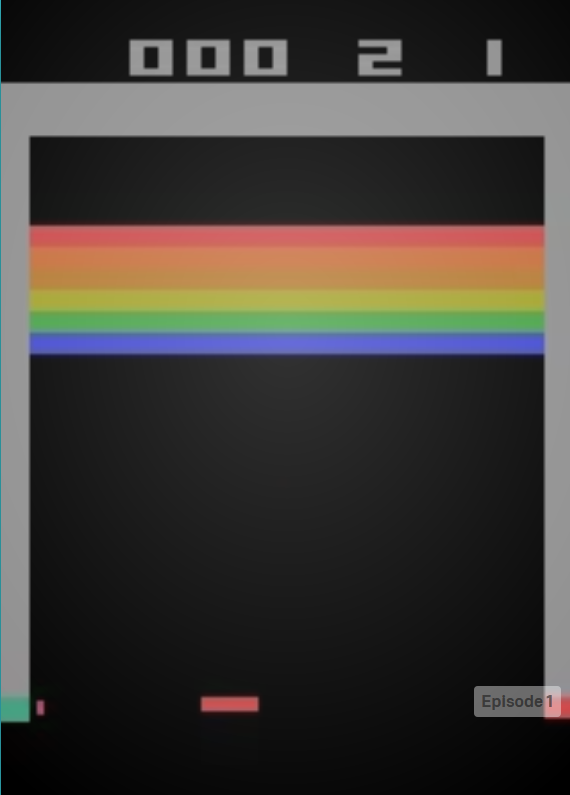
\includegraphics[width=\linewidth, height=0.2\textheight, keepaspectratio]{breakout.png}
    \caption{Sample Atari\texttrademark{} Breakout Game with Random Agent~\autocite{breakout}}~\label{fig:breakout}
\end{figure}

\section{Description of the Question}
As previously mentioned for our term project, we wish to design and train a deep neural network that can play the nostalgic Atari\texttrademark{} Breakout game. The agent is expected to have an ``understanding'' of game mechanics such as how to score, and what moves to avoid. Essentially the agent is expected to have a functioning Atari\texttrademark{} skills.
A set of rewards and punishments, which are associated with certain in-game actions and outcomes, will be used to train the model who play the game over and over again.
At each epoch the artificial intelligence should be a better ``gamer'' than the previous one.

\section{Milestone}
We are planning to conduct a research about reinforcement learning, deep neural networks and more specific algorithms like Deep Q-networks (DQN) that combines Q-learning with deep neural networks to let reinforcement learning to be applied to complex, high dimensional environments, like video games~\autocite{openai}. Furthermore, we are planning to obtain a working, playable version of the Breakout game which is suitable for training and testing our artificial agent.

\printbibliography{}
\end{document}
